\documentclass{article}
    % General document formatting
    \usepackage[margin=0.7in]{geometry}
    \usepackage[parfill]{parskip}
    \usepackage[utf8]{inputenc}
    
    % Related to math
    \usepackage{amsmath,amssymb,amsfonts,amsthm}
\usepackage{graphicx}
%\usepackage{subfig}
%\usepackage{subfigure}
\usepackage{caption}
\usepackage{subcaption}
\usepackage{listings}
\usepackage{braket}
\usepackage{gensymb}
\usepackage[percent]{overpic}
\usepackage{xcolor,varwidth}

\usepackage{titling}
%\usepackage{lipsum}

\usepackage{titlesec}

\titleformat*{\section}{\Large\bfseries}
\titleformat*{\subsection}{\large\bfseries}
%\titleformat*{\subsubsection}{\large\bfseries}
%\titleformat*{\paragraph}{\large\bfseries}
%\titleformat*{\subparagraph}{\large\bfseries}
\titlespacing\section{0pt}{12pt plus 4pt minus 2pt}{0pt plus 2pt minus 2pt}
\titlespacing\subsection{0pt}{12pt plus 4pt minus 2pt}{0pt plus 2pt minus 2pt}
\titlespacing\subsubsection{0pt}{12pt plus 4pt minus 2pt}{0pt plus 2pt minus 2pt}

\pretitle{\begin{center}\large\bfseries}
\posttitle{\par\end{center}\vskip 0.01em}
\preauthor{\begin{center}\Large\ttfamily}
\postauthor{\end{center}}
\predate{\par\normalsize\centering}
\postdate{\par}

\begin{document}

%\maketitle

\begin{center}
\textbf{\LARGE{\centering{Deep Learning}}}\\

\textit{USN: 303039534}\\
\end{center}

\section*{A}

\subsection*{1}

A true perceptron is a binary classifier; we therefore arbitrarily assign the set of vectors for which sum is 0 to the +1 state.

We implement a two-state perceptron with weights \textbf{w} and inputs \textbf{u} such that the state of the perceptron $v$ is given by

\begin{equation}
\begin{split}
+1 \,\,\, {\bf w \cdot u} - \gamma \geq 0 \\
-1 \,\,\, {\bf w \cdot u} - \gamma < 0
\end{split}
\end{equation}

Where $\gamma$ is a threshold parameter. Discuss case where $\gamma = 0$.

We train this perceptron using three different learning rules.
\begin{enumerate}
\item
The Hebbian learning rule
\begin{equation}
{\bf w} = \dfrac{1}{N_\mu} \sum_{m = 1}^{N_S}{v^m {\bf u}^m}
\end{equation}
Where $N_\mu$ is the dimensionality of the space(here 10), $N_S$ is the number of input patterns, and $v^m$ is the desired output for pattern $m$ with input ${\bf u}^m$.

\item
The perceptron learning rule.
\begin{equation}
{\bf w} \rightarrow {\bf w} + \dfrac{\epsilon_w}{2}(v^m - v({\bf u}^m)) {\bf u}^m
\end{equation}
\begin{equation}
\gamma \rightarrow \gamma - \dfrac{\epsilon_w}{2}(v^m - v({\bf u}^m))
\end{equation}
Where $\epsilon_w$ is the learning rate, ,  $v({\bf u}^m)$ is the predicted perceptron state for input $m$, and the other parameters are as above. Although I should probably fix gamma here?

\item
The delta learning rule. 
\begin{equation}
{\bf w} \rightarrow {\bf w} - \epsilon_w \nabla_w E
\end{equation}
If we let $f(s)=\text{tanh}(ax) ~ a \rightarrow \infty$ we have ${\bf f} = {\bf u}$ and can write 
\begin{equation}
E = \dfrac{1}{2} \sum_{m=1}^{N_S}{(v^m-v({\bf u}^m))^2}
\end{equation}
And thus
\begin{equation}
 \nabla_w E = - \sum_{m=1}^{N_S}{(v^m-v({\bf u}^m)) {\bf u}^m}
\end{equation}
This is entirely equivalent to a batch-version of the perceptron learning rule although the derivation of the delta rule requires the use of derivatives that are not strictly possibly for the perceptron learning rule.
Where $N_\mu$ is the dimensionality of the space(here 10), $N_S$ is the number of input patterns, and $v^m$ is the desired output for pattern $m$ with input ${\bf u}^m$.

\end{enumerate}


As explained in Dayan adn Abbott, Hebbian learning depends on $N_u / (N_S - 1)$. Here this ratio is $???$
The perceptron learning rule ensures linear seperation of the input data if this is possible.

we are asked to classify the input based on the sign of the sum. However, this is undefined when the input has 5 elements of +1 and 5 elements of -1. We can approach this in two ways. Either we include a third state '0' for our perceptron and train a three-state model, or we arbitrarily assign the set of vectors for which the sum is 0 to the +1 or -1 category.

Since the perceptron takes binary inputs, building multilayer networks requires the input to be binary, and we therefore opt for the second approach for consistency. We thus classify input vectors for which the sum is 0 as having a positive sign. In practice, we achieve this by letting $\lambda = -0.5$.

Note that there are only $2^10 = 1024$ possible input vectors. 

(test performance as a function of sum)


\begin{figure}[h]
	\centering
	\begin{subfigure}[t]{0.62\linewidth}
		\centering
		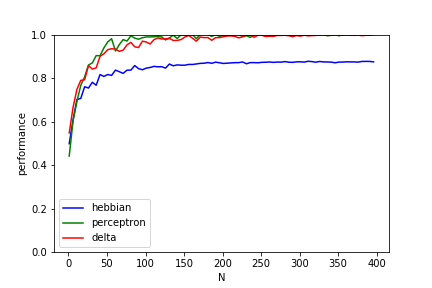
\includegraphics[width = 1.0\linewidth, trim={0 0 0 0}, clip=true]{figures/compare_sum.png}
		\subcaption{Reference}
		%\label{}	
	\end{subfigure}%
\caption{performance for different numbers of positive elements}
\label{fig:nplus}
\end{figure}

\begin{figure}[h]
	\centering
	\begin{subfigure}[t]{0.32\linewidth}
		\centering
		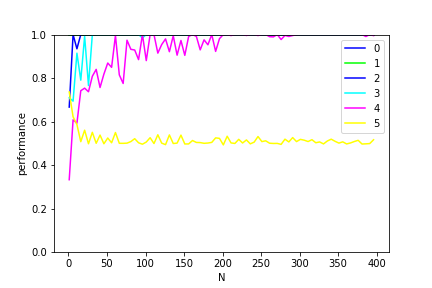
\includegraphics[width = 1.0\linewidth, trim={0 0 0 0}, clip=true]{figures/nplus_heb.png}
		\subcaption{Reference}
		%\label{}	
	\end{subfigure}%
	\hspace{0.01 \linewidth}
	\begin{subfigure}[t]{0.32\linewidth}
		\centering
		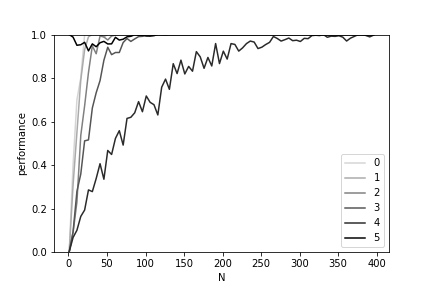
\includegraphics[width = 1.0\linewidth, trim={0 0 0 0}, clip=true]{figures/nplus_perceptron.png}
		\subcaption{No CNV}	
		%\label{}
	\end{subfigure}%
	\hspace{0.01 \linewidth}
	\begin{subfigure}[t]{0.32\linewidth}
		\centering
		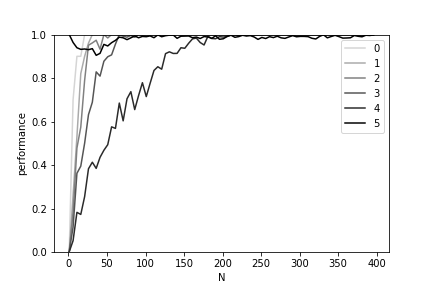
\includegraphics[width = 1.0\linewidth, trim={0 0 0 0}, clip=true]{figures/nplus_delta.png}
		\subcaption{No CNV}	
		%\label{}
	\end{subfigure}%
\caption{performance for different numbers of positive elements}
\label{fig:nplus}
\end{figure}

delta:

new nplus: 0
1
new nplus: 1
4
new nplus: 2
5
new nplus: 3
10
new nplus: 4
27
new nplus: 5
14
new nplus: 6
0


perceptron:

new nplus: 0
3
new nplus: 1
4
new nplus: 2
6
new nplus: 3
11
new nplus: 4
46
new nplus: 5
3
new nplus: 6
0


hebbian:

new nplus: 0
0
new nplus: 1
1
new nplus: 2
2
new nplus: 3
5
new nplus: 4
23
new nplus: 5
100
new nplus: 6
26

\begin{figure}[h]
	\centering
	\begin{subfigure}[t]{0.62\linewidth}
		\centering
		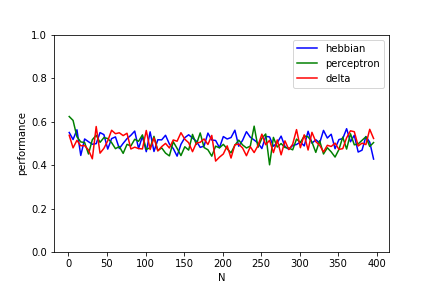
\includegraphics[width = 1.0\linewidth, trim={0 0 0 0}, clip=true]{figures/compare_prod.png}
		\subcaption{Reference}
		%\label{}	
	\end{subfigure}%
\caption{performance for different numbers of positive elements}
\label{fig:nplus}
\end{figure}


Difficult for product since this is not a linearly separable problem; no matter where we draw our line, we will only correctly classify a subset of the inputs. Performance thus saturates near 50\%.

\begin{figure}[h]
	\centering
	\begin{subfigure}[t]{0.32\linewidth}
		\centering
		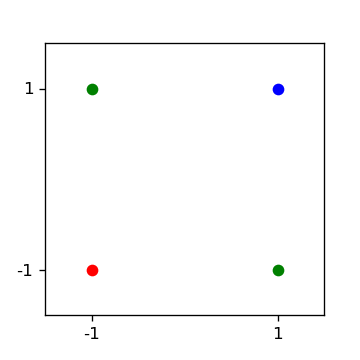
\includegraphics[width = 1.0\linewidth, trim={0 0 0 0}, clip=true]{figures/sum_2d.png}
		\subcaption{Reference}
		%\label{}	
	\end{subfigure}%
	\hspace{0.01 \linewidth}
	\begin{subfigure}[t]{0.32\linewidth}
		\centering
		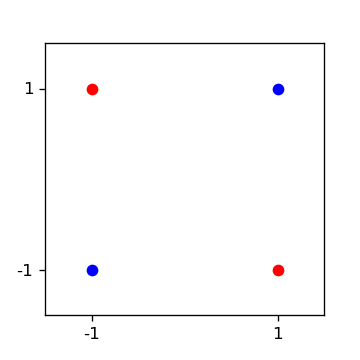
\includegraphics[width = 1.0\linewidth, trim={0 0 0 0}, clip=true]{figures/prod_2d.png}
		\subcaption{No CNV}	
		%\label{}
	\end{subfigure}%

\caption{performance for different numbers of positive elements}
\label{fig:nplus}
\end{figure}

\subsection*{Multi-layer perceptron}

To implement our multi-layer perceptron, we need a differentiable transfer function and choose tanh for consistency with the above step function which corresponds to the tanh function in the limit of infinite scaling.

\begin{figure}[h]
	\centering
	\begin{subfigure}[t]{0.32\linewidth}
		\centering
		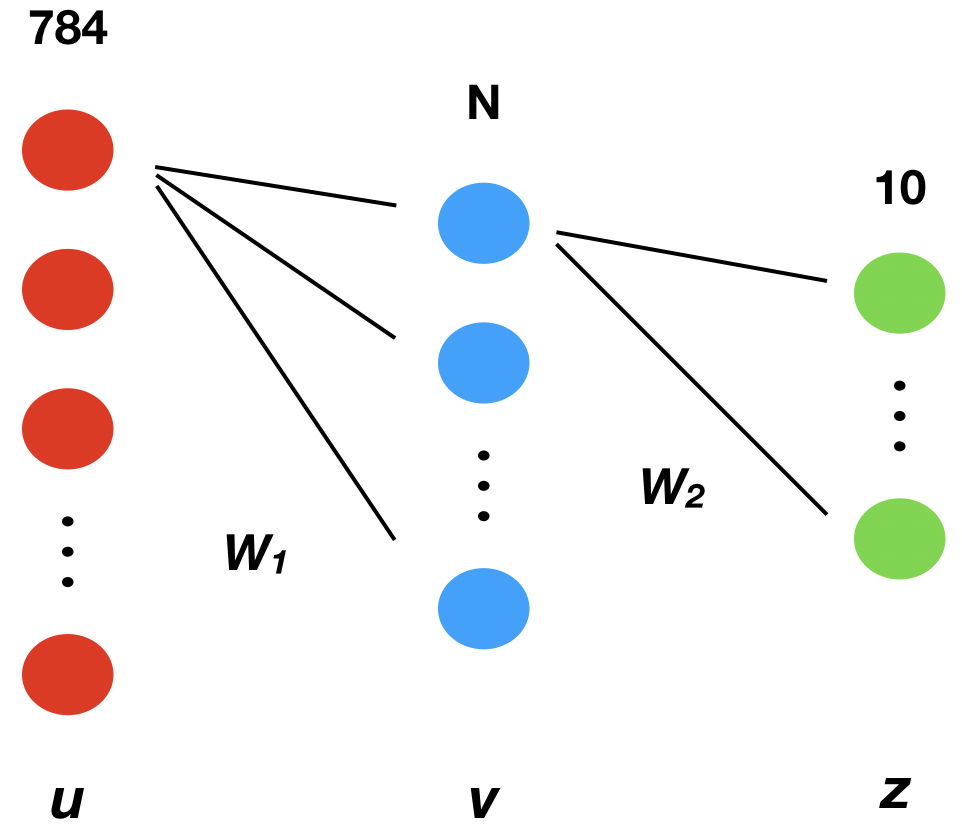
\includegraphics[width = 1.0\linewidth, trim={0 0 0 0}, clip=true]{figures/network_structure.png}
		\subcaption{Reference}
		%\label{}	
	\end{subfigure}%
\caption{performance for different numbers of positive elements}
\label{fig:nplus}
\end{figure}

\begin{equation}
{\bf v} = f( {\bf u W_1} )
\end{equation}

\begin{equation}\label{eq:layer2}
{\bf z} = f( {\bf v W_2} )
\end{equation}

Where $\bf{W}_1$ is a 784xN matrix and $\bf{W}_2$ is an Nx10 matrix, $f$ denotes element-wise application of the tanh() function.

define error function
\begin{equation}
E = \dfrac{1}{2} \sum_k{(t_k - z_k)}
\end{equation}

We want $\Delta w_{ij} = - \eta \dfrac{\partial E}{\partial w_{ij}}$. 

For the second set of weights ${\bf W}_2$, we can derive using the chain rule and equation \ref{eq:layer2}

\begin{equation}
\dfrac{\partial E}{\partial w_{jk}} = -(t_k - z_k)f'(\sum_j{w_{jk}v_j})v_j
\end{equation}

For the tanh function $f'(x) = 1- f(x)^2$ and we can thus use the values of tanh we used in the forward pass to also calculate the weight changes in our backpropagation step; i.e. $f'(\sum_j{w_{jk}v_j}) = 1 - z_k^2$

For the first layer of weights ${\bf W}_1$, we can write

\begin{equation}
\dfrac{\partial E}{\partial w_{ij}} = - u_i f'(\sum_j{w_{ij}u_i}) \sum_k{[(t_k - z_k)f'(\sum_j{w_{jk}v_j})w_{jk}]}
\end{equation}

\begin{equation}
\dfrac{\partial E}{\partial w_{ij}} = - u_i (1 - v_j^2) \sum_k{[(t_k - z_k)(1 - z_k^2)w_{jk}]}
\end{equation}


\end{document}

